\chapter{The Phonemic Model of Language}
\epigraph{En matière de langue on s’est toujours contenté d’opérer sur des unités mal définies (In language's matter it has always been sufficient to operate on ill-defined units).}{Ferdinand de Saussure (1916)}

The sound structure of languages is under the main focus of phonology. Under the phonological point of view, it is not restricted to the sounds at the physical level of speech realization, but also extended to the symbolic `sounds', which are cognitive abstractions that provide a mean of representation for a language.

The `sound' as a physical phenomenon is a complex pattern of disturbance that travels across all forms of matter: gases, liquids, solids, and plasmas; in this context, called the medium. In speech communication, the sound source, the emitter, through its oral tract, produces a disturbance that travels in the free air medium. This disturbance suffers scattering, attenuation and other sorts of distortion as it travels across the medium. The striking force of the disturbance reaches the receptor's ear, what causes, after a series of transformations in the outer, middle and inner ear, neural signals that are sent to the brain and perceived as speech sounds, eliciting meaning and creating communication.

In order to establish a phonemic model of language it is necessary to define which are those cognitive symbols and the rules under which they interact to create a cognitive representation of speech. The Swiss linguist Ferdinand de Saussure is responsible for shifting the way linguistics was done and established a break point with his posthumous publication \textit{Course in General Linguistics} in 1916. Structural linguistics was the new approach to linguists and the creation of phoneme was the basis for all the new born linguistics. To collect a corpus of utterances and to produce an attempt to classify all of the elements of the corpus at their different linguistic levels was the new paradigm that brought linguistics from diachronic to synchronic analysis.

As pointed out by \cite{capek1983}: ``Saussure did not discover -- or invent -- the phoneme. He was one of a number of scholars working on comparable ideas. His statements are important not so much for the accuracy with which they report facts or for their strength and consistency as for the explanatory power of the inferential network they set up. Suffice it to say that after Saussure the clumsy terminology used by scholars who preceded him -- that of speech sounds (\textit{Sprachlaute})  -- came to be replaced by the much more intuitively satisfactory concept of the phoneme.''

The idea of phoneme comes from the idea of minimal differences that elicits meaning. It is regarded as the smallest segment unit in speech that makes meaningful contrast between two utterances. 
Each language has its own phoneme inventory, for example, in English \textipa{/t/} and \textipa{/d/} are distinct phonemes because a simple change from \textipa{/to/} to \textipa{/do/} creates a meaning difference. 
The languages of the world have different sets of phonemes, or, more appropriately, we may say that they have different categorizations. In English no distinction is made between aspirated and unaspirated sounds. 
In Hindi such distinction exists: \textipa{/tal/} 
(beat) contrasts with \textipa{/t\super hal/} (plate) \citep{ladefoged1996}. 
Implicit in the idea of phoneme is that language may be segmented into a sequence of consecutive symbols in time; those segments may be differentiated one from the other; and different symbols create the possibility of different meaning, according to the context in which they are inserted. 
Beno\^it Mandelbrot showed in his paper \citep{mandelbrot} that speech, in order to be comprehensible in the most variate situations and under heavy corruption, must necessarily, at a certain level, be understood as a discrete process, because only in this manner it would make speech comprehension possible in such degenerated situations. Another advantage of the discrete aspect of language is that discreteness at the phonetic level guarantees the discreteness at all other levels, and that is the base of all linguistic knowledge nowadays. 

``Man could not perceive speech well if each phoneme were cued by a unit sound''\citep{liberman1967}. The acoustic cues in an utterance carry information in parallel about successive abstract units, the phonemes. It builds a complex relation between cues and phonemes, and it makes speech perceiving rate slower but also more robust. \cite{liberman1967} pointed some reasons why a speech code could not be alphabetic, a one-to-one correspondence between codes and phonemes. If man can follow a speech at a rate of 400 words per minute, and if each word has an average of 4 to 5 phonemes, that would lead to 30 phonemes per second, what would overrun the human temporal resolving power of sound stimuli \citep{miller1948}. It evidences the necessity to have a surjective mapping\footnote{Surjective mapping is a map from one set onto another set, so that its range is the entire second set.} from acoustic cues into phonological abstract elements. Other acoustic alphabetical codes used for communication have shown that it is hard to achieve a communication rate near the speech rate. The simple example of Morse code shows how ineffective this type of communication is, where the highest rate ever achieved by a skilled operator was 75.2 words per minute \citep{pierpont2002}. Other codes, used in reading devices for the blind (the Optophone, built by Fournier d'Albe in 1913; the Optacon, by John Linvill in 1962; the Stereotoner in 1973 by the Mauch Laboratories; among other examples) were tested, and none showed a performance near the speech communication rate. Another drawback posed by the alphabetic approach is the difficulty of identification of numerous and distinct acoustic stimuli. The works of \cite{miller1956,pollack1952} among others suggest that this number is considerably less then 31, which is the the average number of phonemes in a language (the language with more phonemes is !Xu, spoken in southern Africa, with 141 phonemes; and the languages with fewer phonemes have only 10, the Pirah\~a, spoken by indigenous people in Brazil, and the Rotokas, spoken by a few people in Bougainville, an island to the east of New Guinea \citep{maddieson1884}).

The chief problem in determining the form and behavior of phonemes in a certain language system is to achieve a method of quantitative comparison between two or more phonemes. We may describe speech sounds by their place and manner of articulation, we may extract some of their acoustic characteristics and we may determine whether two sounds build a phonemic contrast in a language, but it is still hard to establish a significant quantitative dissimilarity measure of two phonemes and then discover a unique scale under which all phonemes might be measured. 

Any speech sound production may be described as a sequence of articulatory gestures. Imagine that we take an X-ray moving picture of a person speaking and build a slow-motion picture of the activity of the speech organs during the utterance production. We might then describe in details the articulatory gestures. Suppose for example we are analyzing the utterance of a \textipa{[t]}. We might see the tip of the tongue rising to the top of the back of the upper teeth, forming an occlusion and releasing it. If we analyze the utterance of a \textipa{[d]} instead, the description of the gestures would be quite similar, but added by a contraction, vibration and relaxation of the vocal cords to produce voicing.

As pointed out by \cite{zipf1949}, ``the point of concern at present, however, is not to devise a system of symbols whereby the sequence of sub-gestures constituting a speech-sound can be noted, but rather to remark that speech-sounds and phonemes may be viewed as constellations, or configurations, of articulatory sub-gestures, arranged partly or completely in sequential order, some sequences running concurrently with others (e.g. the occlusion is concurrent with the voicing of \textit{d}). Although there is not a single speech-sound, or variant form, of a phoneme in any language which cannot be conceived of as a constellation or configuration of the type envisaged above, yet a complete and accurate description of even a single speech-sound in terms of sequences is practically impossible. However, by conceiving phonemes as constellations of this order, we have found a very useful method of comparing a number of specific phoneme pairs which have essential sequences in common.''

\cite{zipf1949} proposes that the frequency a phoneme in a language occurs is inversely proportional to its complexity. He analyzed aspirated and unaspirated stops in four languages: Peipingese Chinese, Danish, Cantonese Chinese and Burmese. The data analyzed corroborated his hypothesis. He also analyzed the occurrence of voiced and voiceless stops in twelve languages (Czechish, Dutch, French, Italian, English, Hungarian, Bulgarian, Russian, Spanish, Greek, Latin and Sanskrit) and concluded that the voiceless stop is more frequent then its voiced counterpart. When he compared the occurrence (in German and Sanskrit) of long vowels against short vowels and diphthongs against each of its parts alone, he once again found that the simple one (short single vowel) has a greater frequency of occurrence compared to the complex counterpart (long vowel or diphthong). Comparing also the occurrence of \textipa{[m]} and \textipa{[n]} across 21 languages, he observed that \textipa{[n]} was more frequent. ``It might be taken as some evidence that \textit{n} is the simplest of the two phonemes because of the observation of comparative philology which indicates that quite often, when \textit{m} disappears in any of its usages in a given language, it becomes (i.e. `weakens' to) \textit{n} before disappearing''\citep{zipf1949}. A more complete and recent analysis \citep{maddieson1884} shows that the observations of Zipf might be wrong. In a database of 425 languages, the phone \textipa{[m]} is present in 94.2\% of the languages, against only 44.8\% for the phone \textipa{[n]} and 16.9\% for those languages that have both \textipa{[m]} and \textipa{[n]} (the probability of \textipa{[m]} given \textipa{[n]} is 19.6\% and the probability of \textipa{[n]} given \textipa{[m]} is 22.7\%). The explanation could then be the other way around: \textipa{[m]} is simpler then \textipa{[n]}, and it gets more complex before disappearing (it is preferable to keep in the speech repertoire only simple and contrastive symbols). The only way to corroborate this kind of analysis would be by using the information on the usage frequency of these phones, which is unfortunately unavailable. The phenomena of haplology\footnote{Haplology is the elimination of a syllable when two consecutive syllables are identical or similar.} and the Grassmann's law\footnote{The Grassmann's law is a dissimilatory phonological process observed in Ancient Greek and Sanskrit. According to this law, if an aspirated consonant is followed, in the next syllable, by another aspirated consonant, the first one loses the aspiration, reducing the complexity.} are cited by \cite{zipf1949} to exemplify the relation between the change in the pronunciation complexity  and the change in its frequency of occurrence.

In the history of any language, the phonemic system undergoes constant changes that may affect the complexity and occurrence frequency of phonemes. Comparing two different languages with a common ancestral we might notice these changes and their consequences on frequency and usage. As it has been quite generally observed, the emergence of a phonetic change in a certain language's phonemic system is unpredictable. Any phoneme may find itself suddenly unstable and undergoes a change, whether in all occurrences of this phoneme or, for example, only in certain situations restricted to the relative position it presents. These phonemes that suffered change might stay stable or suffer a subsequent change.	According to \cite{zipf1949}, ``though the emergence of phonetic change is apparently capricious, actual phonetic changes seem to fall into four main and orderly types: (1) the so-called \textit{`spontaneous' changes}; (2) the \textit{accentual changes}; (3) the \textit{assimilatory changes}; and (4) the \textit{dissimilatory changes}.

A comparative analysis on the articulation of many given phonemes and phoneme sequences shows that some phonemes are facilitated due to the restrictions on the physiology of the mouth and a contiguous speech tendency. As an example, we clearly understand why it is easier to pronounce a \textipa{[d]} after \textipa{[n]} then after \textipa{[m]}. When we pronounce an \textipa{[n]}, the tongue touches the hard palate just behind the upper teeth and that is also the articulation point for \textipa{[d]}. The pronunciation of \textipa{[m]}, on the other hand, requires a bilabial closure, what is not part of the articulation for \textipa{[d]}. This facilitation process is clearly observed when we analyze the statistics of diphone occurrences in a Language. In English, for example, the occurrence probability of a \textipa{[d]} given that a \textipa{[n]} has occurred adjacently is 34.9\%, much greater then the 1.8\% probability of occurring the same \textipa{[d]} given that an \textipa{[m]} has just occurred. When comparing a pair like \textipa{[ts]} and its reversal \textipa{[st]}, the observed occurrence frequency in English is 5.1\% and 33.3\%, respectively. The only difference between these pairs is in the movement of the tongue tip.

Although we don't have the means to acquire the same sort of information for all languages in the world, we might use the UPSID database \citep{maddieson1884} to verify what is the probability of occurrence of a phone given that the other is present in that language. Concerning the three phones in the previous analysis \textipa{[m,n,d]}, we get the following result: 94.2\% of the languages that have \textipa{[d]} in its repertoire also have \textipa{[m]} in it; 89.2\% of the languages that have \textipa{[d]} in its repertoire also have \textipa{[n]} in it; 26.6\% of the languages that have \textipa{[m]} in its repertoire also have \textipa{[d]} in it; 53.0\% of the languages that have \textipa{[n]} in its repertoire also have \textipa{[d]} in it; 47.0\% of the languages that have \textipa{[m]} in its repertoire also have \textipa{[n]} in it; and 99.0\% of the languages that have \textipa{[n]} in its repertoire also have \textipa{[m]} in it.
% 0.94167 of the languages with d also have m
% 0.89167 of the languages with d also have n
% 0.26588 of the languages with m also have d
% 0.52970 of the languages with n also have d

As another example, consider the occurrence of \textipa{[t]} and \textipa{[d]} between vowels. It is easier to keep the vocal folds vibrating during the whole interval, producing a \textipa{[d]}, than stopping its vibration for a very short time and starting it again, producing then a \textipa{[t]}. \cite{zipf1949} gives as an example the pair \textipa{[p]}-\textipa{[b]}. The Latin word for `river bank' is \textit{ripa}, which became \textit{riba} in Old Provençal, due to this facilitation process. \cite{zipf1949} argues that ``when an intervocalic \textit{p} becomes voiced in a given language, it is an indication rather of the instability of \textit{p} in that given language that of a universal instability of intervocalic \textit{p}; for example, we have for centuries been pronouncing intervocalic \textit{p} in English \textit{rapid}, \textit{tepid}, \textit{paper} without the shifting of \textit{p} to \textit{b}''. Comparing the statistics of occurrence of VCV-like triphones in English, the percentage of V\textipa{t}V is 10.13\% against 5.59\% of V\textipa{d}V; V\textipa{k}V 8.59\% against 2.18\% for V\textipa{g}V; V\textipa{f}V appears 8.36\% and V\textipa{v}V 3.88\%; V\textipa{b}V 5.02\% almost like its voiceless counterpart V\textipa{p}V with 4.70\%. In all the cases presented, except the bilabial one (which shows a very similar frequency of occurrence), the voiceless consonant exhibits a distinguished frequency of occurrence. This result shows a greater stability of the voiceless consonants in English, although it is known that in some dialects of American English there is a tendency towards voicing the intervocalic plosive consonant \textipa{[t]}. ``In these dialects the differences between \textit{latter} and \textit{ladder}, \textit{kitty} and \textit{kiddy}, \textit{metal} and \textit{medal} are practically subliminal; the couplets are distinguished more by the usage of the words than by perceptible differences in the phonemes''\citep{zipf1949}.

The Latin word \textit{ripa} became \textit{riba}, and from that came the word \textit{rive} in French. The Latin \textit{faba} became the French \textit{fève}, ``the intervocalic \textit{p} of Latin began to approximate the norm of \textit{b} to such an extent that in intervocalic positions the two behaved indistinguishably, and subsequently, in losing their explosiveness in this position, both began to approximate the norm of \textit{v}''\citep{zipf1949}. This process of shift suffered by some phonemes is such a slow process that has to be apprised over a considerable extent of time. The statistical analysis of relative frequencies is important to determine the dynamics and evolution of a language. The balance between phonemes and their metamorphosis through time are keys to understand how linguistics categories are built and shaped. It is important to study the processes of assimilation (merge) and differentiation (split) in a language. As pointed by \cite{zipf1949}, ``every assimilation points to a weakening or instability of the assimilated sound, and this weakening or instability is caused primarily by the excessive relative frequency of the assimilated sound''.

One example of differentiation process is found in Germanic languages where the back vowels \textipa{[u]} and \textipa{[o]} were originally in an allophonic relation to \textipa{[y]} and \textipa{[\o]}, respectively, when they are placed before a following vowel \textipa{/i/}. With time, the syllables containing this \textipa{/i/} were lost, and a phonemic split made the phones \textipa{/y/} and \textipa{/\o/} distinct phonemes. Two front rounded phonemes were added to the vowel system repertoire. Analyzing the vowel system in various languages, we observe that most of them have front unrounded vowels or diphthongs (449 languages of all 451 languages in the UPSID database) and only very few languages have front rounded vowels or diphthongs (46 languages in the UPSID databese). This means that only 2 languages have a vowel system built exclusively on front rounded vowels. In the same way, there are 44 languages using a mixed vowel system with front rounded and front unrounded vowels; and 405 languages using an exclusive front unrounded vowels system. An explanation for the reason of this finding is that most languages choose vowels that are maximally distant from one another. Front vowels have a higher second formant (F2) then back vowels; unrounded vowels also have a higher F2 than rounded vowels. This means that unrounded front vowels and rounded back vowels have maximally different second formant, which enhances the differentiation between them. Every dissimilation points to a strengthening of the existing splitting sounds, their excessive relative frequency and their semantic difference build a barrier to create distinction where, before, was a categorical amalgam.

We might wonder that there could exist thresholds of tolerance comprising the relative frequency of phonemes in order to justify or deny the applicability of processes of assimilation or differentiation. Those thresholds are limits to the relative frequency of a phoneme, bellow which a phoneme tends to weaken and above which it tends to strengthen, creating merges and splits. At a first analysis of what might be these thresholds, we have to keep in mind an obvious fact: a sufficient variability is important to create distinct symbols, so that the permutation of them can express the information exchanged during communication. Among the 451 languages in the UPSID databese, the minimum number of segments used by a language is 11, in only two languages (Pirah\~a, spoken in Brazil by around 300 speakers; and Rotokas, spoken in Papua New Guinea by approximately 4,300 speakers). On the other hand, it is also not efficient to have a code with so many symbols, because the probability of false detection would increase so much and make communication unproductive. The language with the highest number of segments found in the UPSID database has 141 segments (the !Xu language, also called !Kung, is spoken by fifteen thousand speakers in Namibia and Angola). On average, the languages are built on 
31 %30.97 
segments. Figure \ref{fig:language_segments_hist} bellow shows the histogram of languages regarding the number of segments used in each of them.

\begin{figure}[h!]
\centering
\includegraphics[width=0.75\textwidth]{images/segments_hist_upsid2.pdf}
\caption{Number of segments in various languages of the world, using the UPSID databese (follows apparently a Rayleigh distribution).}
\label{fig:language_segments_hist}
\end{figure}

The analysis using the CMU Pronouncing Dictionary of English shows that this language has 39 phonemes, not counting variations due to lexical stress. The frequency of occurrence of these phones is presented in Figure \ref{fig:phones_hist_en}. It shows that the most frequent symbol is \textipa{[@]}, accounting 10.12\% of symbols occurrence in that language. Following in order of frequency of occurrence comes \textipa{[t]} with 6.99\% and \textipa{[n]} with 6.92\%. The most infrequent phoneme in English is the diphthong \textipa{[OI]} which occurs with a relative frequency of only 0.1\%. Preceding it is the phoneme \textipa{[U]} with 0.42\% of relative frequency (see chapter \ref{sec:lang_stat} for more information).

\begin{figure}[h!]
%\centering
\noindent\makebox[\textwidth]{%
%\def\svgwidth{1.25\textwidth}
%\input{images/phones_hist_en.eps_tex}
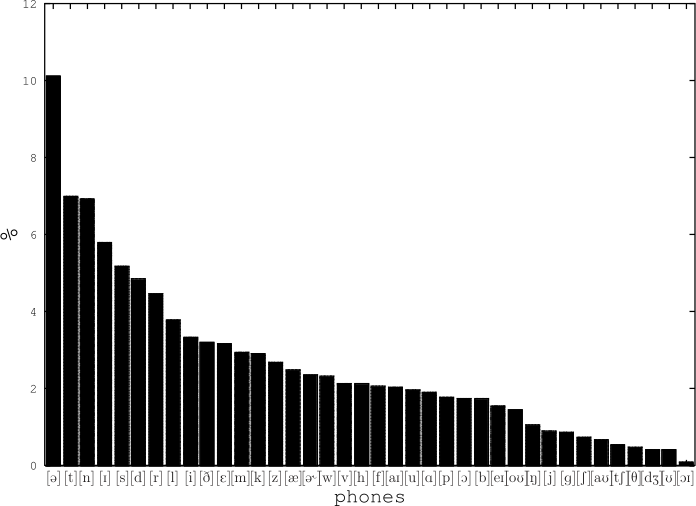
\includegraphics[width=\textwidth]{images/phones_hist_en.pdf}
}
\caption{Frequency of occurrence of English phones.}
\label{fig:phones_hist_en}
\end{figure}

If we had these relative frequencies, during one language evolution, like the previous ones derived for English, they could be used as a first approximation to determine the thresholds for assimilation and dissmilation processes. The phonemes cannot have, all of them, the same percentage-threshold, for the weakening of a phoneme, causing an assimilation process, could lead the target phoneme to an excessive relative frequency, and it would require this target phoneme to be capable of sustaining a higher frequency then the vanishing one. It is quite reasonable to consider that phonemes have distinct thresholds, what might be explained by their different acoustic and usage properties. It would be necessary to apprise and compare the features of phonemes, and also the way they are used and connected to build utterances.

According to \cite{zipf1949}, when a phoneme become so rare, with a relative frequency abnormally low, ``the phoneme then would become a distinctive and very characteristic part of every word in which it occurred''. In such situations, an accidental epenthesis might appear, like the strengthening of \textipa{[t]} into \textipa{[ts]} observed in the Old-High-German sound-shift in which a Germanic \textipa{[t]} shifted to a \textipa{[ts]} in the majority of positions, and it went even further in some cases to \textipa{[ss]}. Some examples in German, compared to the English counterpart, which preserved the \textipa{[t]}, are: \textit{zwei}, \textit{two}; \textit{zehn}, \textit{ten}; \textit{zug}, \textit{tug}; \textit{zahn}, \textit{tooth}; \textit{zeit}, \textit{time}.

Observing 12 languages, \cite{zipf1949} concludes that, with a few exceptions 
(the Spanish \textit{d} and \textit{t}, and the Hungarian \textit{b} and \textit{p}), 
the voiceless stops strongly outnumber their voiced counterparts and the relative frequencies 
of occurrence are amazingly similar. Considering that the voicing assimilation is a normal 
process found in many languages, it seems a quite astonishing result. It seems like other factors 
prevent this assimilation process from occurring. We could then consider the hypothesis that voiced 
stops have a lower threshold, and the assimilation process would force them to cross this threshold. 
In this situation, the assimilation would not move forward, and the voiceless stops are in a great number 
preserved.

The temporal nature of speech is evident. During an utterance, a speech context is built, and such a context is capable of influencing how speech is perceived. The perception of a initial sound of \textipa{[k]} or \textipa{[g]} is influenced by the following sounds, \textipa{[Is]} or \textipa{[Ift]}, for example, creating confusion and leading to false identifications (in the case of \textipa{[kIft]} or \textipa{[gIs]}) due to the existence of the words `gift' and `kiss'. The perception of what is currently being uttered both influences and is influenced by the perception of what comes later and what came previously. So, we might think of speech as a memory non-causal process.

Another aspect, as we observe the speech phenomena through time, is that, although we fight to achieve a segmental model of successive speech units, it has not been shown possible to split the speech continuum into a sequence of discrete elements, since the speech cues frequently overlap in time. The schematic problem of the overlap is shown in Figure \ref{fig:liberman}. The problem of overlap is less severe but still exists at word level. In normal speech, mainly in rapid speech, words run into each other. This phenomena is easy to perceive when we are listening to a foreign language and we can't tell when a word ends and another starts. It is not unusual to have speech errors due to wrong segmentation of words, what might be influenced by the context \citep{bondgarnes,cole1980}.

\begin{figure}[h!]
\centering
\includegraphics[width=0.45\textwidth]{images/liberman.png}
\caption{A schematic spectrogram for the word `bag' presenting the overlapping of acoustic cues. \citep{liberman1970}}
\label{fig:liberman}
\end{figure}  

There have been many ideas of how speech perception works and what are the basic units of it. It is still not clear how we segment speech as we perceive or whether we segment it at all. Various researchers advocate in favor of different approaches: \cite{klatt1979} arguments in favor of diphones; \cite{pisoni1982} in favor of phonemes, what seems to be the most accepted view in the literacy; \cite{fujimura1978} argues in favor of demisyllable; \cite{wickelgren1969} is in favor of context-sensitive allophones; and \cite{studdert1976} is in prol of using syllables as basic units. It seems reasonable to take the advantages of each approach and overcome each of their drawbacks, to take the problem under a multi-resolution point of view. It would, at a first glance, increase the complexity of the model.


The cues not only overlap one into another, but they also are different according to the various context they may appear. As presented by \cite{liberman1967}, the second-formant transition is responsible for determining what consonant the listener perceives. Figure \ref{fig:liberman2} presents some results for different transitional patterns for the second-formant.

\begin{figure}[h!]
\centering
\includegraphics[width=0.75\textwidth]{images/liberman2.png}
\caption{The second-formant starts at, or points to, the \textipa{/d/} locus. On (a), the syllables were perceived as \textipa{/b/}, \textipa{/d/} or \textipa{/g/}, depending on the final frequency level of the formant. On (b), all syllables were perceived as beginning with \textipa{/d/}. \citep{liberman1967}}
\label{fig:liberman2}
\end{figure} 
